\section{Date: 2024-10-18}
\noindent \textbf{Series ID: BRVSLV02JPQ460S} 

\noindent This series is titled Business Tendency Surveys: Volume of Stocks: Economic Activity: Retail Trade, Except of Motor Vehicles and Motorcycles: Current for Japan and has a frequency of Quarterly. The units are Percentage balance and the seasonal adjustment is Seasonally Adjusted.The observation start date is 1990-10-01 and the observation end date is 2024-04-01.The popularity of this series is 1. \\ 

\noindent \textbf{Series ID: CIU2016000000000I} 

\noindent This series is titled Employment Cost Index: Total compensation for Private industry workers in Education and health services and has a frequency of Quarterly. The units are Index Dec 2005=100 and the seasonal adjustment is Not Seasonally Adjusted.The observation start date is 2001-01-01 and the observation end date is 2024-04-01.The popularity of this series is 0. \\ 

\subsection{Regression Tables and Plots}
\begin{center}
\begin{tabular}{lclc}
\toprule
\textbf{Dep. Variable:}               & value\_fred\_CIU2016000000000I & \textbf{  R-squared:         } &     0.491   \\
\textbf{Model:}                       &              OLS               & \textbf{  Adj. R-squared:    } &     0.485   \\
\textbf{Method:}                      &         Least Squares          & \textbf{  F-statistic:       } &     88.72   \\
\textbf{Date:}                        &        Fri, 18 Oct 2024        & \textbf{  Prob (F-statistic):} &  3.81e-15   \\
\textbf{Time:}                        &            10:29:03            & \textbf{  Log-Likelihood:    } &   -384.76   \\
\textbf{No. Observations:}            &                 94             & \textbf{  AIC:               } &     773.5   \\
\textbf{Df Residuals:}                &                 92             & \textbf{  BIC:               } &     778.6   \\
\textbf{Df Model:}                    &                  1             & \textbf{                     } &             \\
\textbf{Covariance Type:}             &           nonrobust            & \textbf{                     } &             \\
\bottomrule
\end{tabular}
\begin{tabular}{lcccccc}
                                      & \textbf{coef} & \textbf{std err} & \textbf{t} & \textbf{P$> |$t$|$} & \textbf{[0.025} & \textbf{0.975]}  \\
\midrule
\textbf{const}                        &     138.6274  &        2.544     &    54.495  &         0.000        &      133.575    &      143.680     \\
\textbf{value\_fred\_BRVSLV02JPQ460S} &      -1.7169  &        0.182     &    -9.419  &         0.000        &       -2.079    &       -1.355     \\
\bottomrule
\end{tabular}
\begin{tabular}{lclc}
\textbf{Omnibus:}       &  2.430 & \textbf{  Durbin-Watson:     } &    0.195  \\
\textbf{Prob(Omnibus):} &  0.297 & \textbf{  Jarque-Bera (JB):  } &    1.900  \\
\textbf{Skew:}          & -0.191 & \textbf{  Prob(JB):          } &    0.387  \\
\textbf{Kurtosis:}      &  2.418 & \textbf{  Cond. No.          } &     23.6  \\
\bottomrule
\end{tabular}
%\caption{OLS Regression Results}
\end{center}

Notes: \newline
 [1] Standard Errors assume that the covariance matrix of the errors is correctly specified.

\begin{figure}
\centering
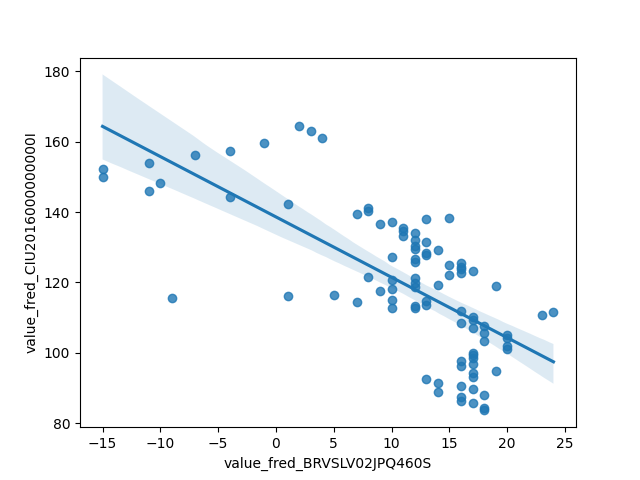
\includegraphics[scale = 0.9]{plots/plot_2024-10-18.png}
\caption{Regression Plot for 2024-10-18}
\end{figure}
\newpage
